% =================================================================
% Scientific Reports (Nature Portfolio) submission manuscript
% Adaptive Multi-Objective Chaotic S-Box Design for Lightweight and
% Secure IoT Communication
%
% Self-contained: inline bibliography (no .bbl / .bib / .bst needed).
% Compile with: pdflatex main_Scientific_Reports.tex
% =================================================================

\documentclass[11pt,a4paper]{article}

% --- Packages allowed on Nature's TeX Live 2025 server -------------
\usepackage[T1]{fontenc}
\usepackage[utf8]{inputenc}
\usepackage{lmodern}
\usepackage[margin=2.5cm]{geometry}
\usepackage{lineno}                % line numbers for review
\usepackage{fancyhdr}              % footer page numbers
\usepackage{graphicx}
\usepackage{amsmath,amssymb}
\usepackage{booktabs}
\usepackage{array}
\usepackage{multirow}
\usepackage{caption}
\usepackage{setspace}
\usepackage{enumitem}
\usepackage[hidelinks,breaklinks=true]{hyperref}

% --- Page style: page numbers in footer, line numbers throughout ---
\linenumbers
\pagestyle{fancy}
\fancyhf{}
\renewcommand{\headrulewidth}{0pt}
\fancyfoot[C]{\thepage}
\setlength{\parskip}{0.6\baselineskip plus 0.2\baselineskip minus 0.1\baselineskip}

\sloppy

% --- Title page metadata ------------------------------------------
\title{\normalsize Adaptive Multi-Objective Chaotic S-Box Design for Lightweight and Secure IoT Communication}

\author{
R. Saktheeswari$^{1}$, Ranjith Raj Anbalagan$^{2}$,\\
Aravind Pitchai Venkataraman$^{3}$, Kehali Anteneh Jember$^{4,\ast}$\\[0.4em]
\small $^{1}$Department of IT, Sri Venkateswara College of Engineering,\\Pennalur, Sriperumbudur 602117, Tamil Nadu, India.\\
\small $^{2}$Department of Production Engineering, NIT Tiruchirappalli 620015, Tamil Nadu, India.\\
\small $^{3}$St.\ Joseph College of Engineering, St.\ Joseph University in Tanzania, Dar es Salaam, Tanzania.\\
\small $^{4}$Department of Electronics and Communication Engineering, Adama Science \& Technology University, Adama, Ethiopia.\\
\small $^\ast$Corresponding author. Email: \texttt{Kehali.anteneh@astu.edu.et}
}

\date{}

\begin{document}

\maketitle

% =================================================================
% Abstract (unstructured, ≤ 200 words, no references)
% =================================================================
\begin{abstract}
Substitution boxes (S-boxes) are nonlinear components used in many
symmetric ciphers, but their security properties must be evaluated
independently of any complete encryption scheme. We study a deterministic
Fisher--Yates permutation generator driven by a coupled two-dimensional
Logistic map and compare NSGA-II with and without periodic Flower
Pollination Algorithm (FPA) perturbations. The optimizer uses three
independent objectives: largest Lyapunov exponent, minimum coordinate
nonlinearity, and differential uniformity. Avalanche and linear-approximation
metrics are calculated after optimization. In five paired simulation
seeds, mean selected minimum nonlinearity was 102.0 (SD 0.00) for FPA
and 102.0 (SD 1.41) for NSGA-II-only; mean differential uniformity was
10.0 (SD 0.00) for both variants. Exact paired tests
with Holm correction detected no statistically supported differences
in the reported metrics. The corrected Lyapunov estimates are on the expected scale
(approximately 0.67--0.69 for the selected solutions), not the previously
reported values near 16.8. The final selected LE range was
0.666--0.682. The study is simulation-only: no complete
cipher or target-device timing is evaluated, and the results do not
establish suitability for deployment.

\end{abstract}

\paragraph*{Keywords:}
Multi-objective optimization; NSGA-II; Chaotic Map; Substitution Box;
Lightweight Cryptography; Internet of Things.

% =================================================================
% 1. Introduction
% =================================================================
\section{Introduction}
\label{sec:intro}

Substitution boxes (S-boxes) provide the nonlinear component in many
symmetric-key ciphers. Their evaluation commonly includes Boolean
nonlinearity, avalanche behavior, differential uniformity, and linear
approximation bias; these criteria capture distinct structural
properties and should not be conflated with the security of a complete
cipher~\cite{adams2010goodsboxes, carlet2020indicator}
\cite{matsui1993linear, biham1991differential}. Chaotic-map-driven
permutation generation and evolutionary search have both been studied
as construction approaches~\cite{cassalquiroga2019generationofdynami, kuznetsov2024evolutionaryapproa}
\cite{mclaughlin2013usingevolutionaryc}.

Prior chaotic S-box studies have explored map-driven permutation
construction and evolutionary search, but comparisons depend on the
specific map, objective definitions, and evaluation protocol. For this
reason, we focus here on a controlled, reproducible comparison of two
search variants under the same implementation and seed schedule rather
than claiming superiority over the literature.

We implement an NSGA-II search on parameters of a modulo-one
coupled Logistic map and compare it with the same search augmented by
periodic Flower Pollination Algorithm (FPA) perturbations. The search
uses three independent objectives: largest Lyapunov exponent, minimum
coordinate nonlinearity, and differential uniformity. We evaluate SAC,
BIC-SAC deviation, and linear approximation probability after
optimization; they are not part of the fitness vector. Our five-seed
comparison is exploratory and does not demonstrate a statistically
supported advantage for FPA.

The rest of the paper is organised as follows.
Section~\ref{sec:methods} develops the 2D Logistic map, the
map-to-permutation construction, the multi-objective fitness
formulation, and the NSGA-II--FPA hybrid.
Section~\ref{sec:results} reports the corrected Pareto search,
post-hoc S-box metrics, and the paired five-seed ablation.
Section~\ref{sec:discussion} interprets the simulation-only evidence
and its limitations. Section~\ref{sec:conclusions} summarises the
findings and identifies the experiments required next.

% =================================================================
% 2. Materials and Methods
% =================================================================
\section{Materials and Methods}
\label{sec:methods}

\paragraph{Notation.}
We treat an 8-bit S-box as a permutation $S:\{0,1\}^8 \to \{0,1\}^8$.
Let $x_n, y_n \in [0, 1)$ be the state variables of the modulo-one
2D Logistic map. The optimizer searches phase genes
$p_x,p_y\in[0,1)$ and maps them to valid initial states by
$x_0=\sin^2(\pi p_x)$ and $y_0=\sin^2(\pi p_y)$. The control
parameters satisfy $\mu\in[3.57,4.0)$ and $\gamma\in[0,0.5)$. Let
$\chi_\mathrm{LE}$ denote the largest Lyapunov exponent, $\mathrm{NL}$
the minimum per-coordinate nonlinearity, $\mathrm{DU}$ the
differential uniformity, $\mathrm{LAP}$ the linear approximation
probability, $\mathrm{SAC}$ the strict avalanche criterion, and
$\mathrm{BIC}_\mathrm{SAC}$ the BIC-SAC deviation from $0.5$. These
metrics follow the canonical S-box evaluation framework of
\cite{adams2010goodsboxes, carlet2020indicator}
\cite{matsui1993linear, nyberg1993perfect}
\cite{biham1991differential, carlet2020indicator}.

\paragraph{Two-dimensional Logistic map.}
The 2D Logistic map is a coupled quadratic iteration with a single
nonlinearity parameter $\mu$ and a coupling parameter $\gamma$:
\begin{equation}
  \begin{aligned}
    x_{n+1} &= \mu \cdot x_n \cdot (1 - x_n) + \gamma \cdot y_n \\
    y_{n+1} &= \mu \cdot y_n \cdot (1 - y_n) + \gamma \cdot x_n.
  \end{aligned}
  \label{eq:2dlogistic}
\end{equation}
Equation~\ref{eq:2dlogistic} defines the modulo-one map used in this
simulation. The parameter $\mu$ controls the coordinate nonlinearity,
and $\gamma$ couples the coordinates. When $\gamma=0$, the system
reduces to two independent one-dimensional logistic maps; selected
solutions are therefore checked for proximity to this boundary.

We estimate the largest Lyapunov exponent by iterating a unit tangent
vector $v_n$ under the Jacobian and renormalizing after each step:
\begin{equation}
  v_{n+1}=\frac{J(x_n,y_n)v_n}{\|J(x_n,y_n)v_n\|},\qquad
  \chi_\mathrm{LE}\approx\frac{1}{N}\sum_{n=0}^{N-1}
  \log\|J(x_n,y_n)v_n\|,
  \label{eq:le}
\end{equation}
where $J$ is the Jacobian of the map and an initial transient is
excluded. For $\gamma=0$ and $\mu=4$, the expected largest exponent
is $\log 2$; this provides a numerical sanity check on the implementation.

\paragraph{Map $\rightarrow$ permutation (Fisher--Yates driver).}
We construct an 8-bit permutation by applying Fisher--Yates to the
identity permutation and using successive $x$-coordinates of the
modulo-one map as swap keys. After burning a transient of $T_0=500$
map iterations, one map step supplies each key $k_i\in[0,1)$ for
\begin{equation}
  \begin{aligned}
    \mathrm{perm} &= [\,0, 1, \ldots, 255\,]; \\
    &\quad \text{for } i = 255 \text{ down to } 1: \\
    &\qquad j = \lfloor k_i \cdot (i + 1) \rfloor,\;
    \mathrm{perm}[i] \leftrightarrow \mathrm{perm}[j],
  \end{aligned}
  \label{eq:fy}
\end{equation}
Equation~\ref{eq:fy} produces a deterministic permutation of length
$256$ with no collisions because Fisher--Yates preserves bijectivity
by construction. The chaotic keys are highly sensitive to the
parameters $(x_0, y_0, \mu, \gamma)$, so a small parameter
perturbation yields a structurally different permutation.

\paragraph{Multi-objective fitness.}
We minimize the following three-objective vector:
\begin{equation}
  \mathbf{f}(S; x_0, y_0, \mu, \gamma) =
  \bigl( -\chi_\mathrm{LE},\;
         -\mathrm{NL}_{\min}(S),\;
         \mathrm{DU}(S) \bigr),
  \label{eq:fit}
\end{equation}
The three objectives are independent quantities in the implemented
fitness. SAC, BIC-SAC deviation, and LAP are evaluated after search
and do not affect selection. No runtime or energy measurement is
included in the fitness or reported as a measured device result.

\paragraph{NSGA-II population search.}
The three-objective optimization uses a population $P_t$ of size
$N_\mathrm{pop}=80$, initialized uniformly over phase genes
$[0,1)^2$ and parameter intervals $[3.57,4.0)\times[0,0.5)$. Each generation
performs nondominated sorting, crowding-distance assignment, binary
tournament selection by rank then crowding distance, uniform
per-gene crossover (probability 0.5), Gaussian mutation
($\sigma=0.01$) clipped to the search bounds, and elitist
$(\mu+\lambda)$ survivor selection back to 80 individuals. The run
uses $G=20$ generations.

\paragraph{FPA perturbation ablation.}
For the hybrid variant, every three generations up to ten members of
the first nondominated front, ordered by crowding distance, are
perturbed with the Flower Pollination Algorithm~\cite{yang2012flowerpollination}.
With probability $p=0.8$, a global Lévy-flight perturbation moves the
chromosome relative to a randomly chosen other population member;
otherwise a Gaussian local perturbation is applied. The step uses
Mantegna's construction with $\beta=1.5$ and scale 0.01. The
comparison variant runs the same algorithm and settings with these
perturbations disabled.

\paragraph{Simulator and reproducibility.}
All optimization results are simulated, not measured on physical
hardware. The source code, seed-level JSON outputs, and software
versions are provided with the reproducibility materials. No device
runtime, energy, or side-channel measurements are claimed. All runs
use population size 80, 20 generations, and parameter bounds
phase genes $p_x,p_y\in[0,1)$ mapped as $x_0=\sin^2(\pi p_x)$ and $y_0=\sin^2(\pi p_y)$, $\mu\in[3.57,4.0)$, and $\gamma\in[0,0.5)$;
paired optimizer runs use seeds 42, 100, 1234, 2025, and 7777.

\paragraph{Post-hoc S-box metrics.}
We report minimum and mean coordinate-function nonlinearity,
strict avalanche criterion (SAC), BIC-SAC deviation, differential
uniformity (DU), and linear approximation probability (LAP).
Nonlinearity is computed from the Walsh--Hadamard spectra of the
coordinate Boolean functions. SAC is the mean of the $8\times8$
avalanche-dependence matrix. BIC-SAC deviation is the mean absolute
deviation of pairwise avalanche-bit XOR probabilities from $0.5$.
DU is the maximum nontrivial entry in the $256\times256$
difference-distribution table. LAP is the maximum probability bias
$|\Pr[a\cdot x=b\cdot S(x)]-1/2|$ over nonzero masks $a,b$.
For a bijective 8-bit S-box, output Shannon entropy is exactly 8 bits
by construction and is therefore not treated as an informative result.
NPCR and UACI are omitted because this study does not define or test
a complete encryption scheme; these are not properties of an isolated
S-box.

\paragraph{Comparisons.}
The previous comparison combined 4-bit and 8-bit S-boxes and included
baselines whose implementation and provenance were not sufficiently
documented for a like-for-like comparison. We therefore do not make
quantitative baseline claims in this revision. The reported optimizer
ablation compares NSGA-II with the same implementation augmented by
FPA perturbations, using paired seeds and identical population and
generation budgets.

\paragraph{Software environment.}
The verified reruns used Python 3.12.3, NumPy 1.26.4,
Matplotlib 3.10.8, and SciPy 1.14.1. Each optimizer variant used
population size 80, 20 generations, Gaussian mutation standard
deviation 0.01, and seeds 42, 100, 1234, 2025, and 7777. FPA runs
perturbed up to ten high-crowding members every three generations;
paired NSGA-II-only runs used the same seeds and settings with FPA
disabled. The source and raw JSON outputs are included in the
reproducibility deposit materials.

% =================================================================
% 3. Results
% =================================================================
\section{Results}
\label{sec:results}

The five-seed results in this section were regenerated using the
configuration and source code described above; individual seed outputs
are included in the reproducibility materials.

\paragraph{Lyapunov-exponent scale check.}
For the selected solutions across both variants, the corrected
largest-exponent estimates were between 0.667 and 0.694. At
$\gamma=0$ and $\mu=4$, the map reduces to independent logistic
coordinates and the exponent is close to $\log 2$, as expected.
The previous values near 16.8 resulted from an incorrect tangent
renormalization and are withdrawn.

\paragraph{Paired optimizer comparison.}
We ran NSGA-II and NSGA-II with periodic FPA perturbations under the
same five seeds (42, 100, 1234, 2025, 7777), population size 80,
and 20 generations. Table~\ref{tab:ablation} reports selected
solutions as mean (SD). FPA-minus-NSGA-II-only differences were
$-0.00295$ for LE (95\% paired bootstrap CI [-0.00854, 0.00332]),
$-0.8$ for NL$_{\min}$ ([-1.6, 0.0]), 0.00239 for SAC
([-0.00107, 0.00605]), $-0.00067$ for BIC-SAC deviation
([-0.00199, 0.00066]), 0 for DU ([0,0]), and 0.00625 for LAP
([-0.00469, 0.01719]). Exact paired sign-flip tests with Holm
correction gave adjusted $p=1.0$ for all endpoints. With five seed
pairs, these estimates are imprecise and do not establish superiority
or equivalence. Mean final nondominated-front sizes were 6.0 with FPA
and 4.4 without FPA; this count is descriptive and does not establish
superior front quality.

The selected-solution averages are not a substitute for comparison
of full Pareto-front quality. Future work should use a prespecified
hypervolume or coverage measure and a larger independent seed set.
We make no claim that FPA improves the search.

\paragraph{S-box properties.}
Across five selected solutions per variant, mean
$\mathrm{NL}_{\min}$ was 101.6 (SD 0.89) for FPA and 102.4
(SD 0.89) for NSGA-II-only; mean DU was 10.0 (SD 0) for both.
These 8-bit boxes have lower
$\mathrm{NL}_{\min}$ and higher differential and linear biases than
the standard AES S-box under the same metric implementations. These
properties describe S-boxes only; they do not establish the security
of a complete cipher. No NPCR/UACI or hardware performance results
are reported.

% =================================================================
% 4. Discussion
% =================================================================
\section{Discussion}
\label{sec:discussion}

This study evaluates a simulated S-box construction and a paired
search ablation; it does not evaluate a complete encryption system,
side-channel resistance, or target-device performance. The five-seed
results provide no statistically supported evidence of an FPA benefit.
The corrected Lyapunov estimates are on the expected scale and supersede
the previous values caused by tangent-vector renormalization error.
Selected solutions span $\gamma=0.00045$ to $0.49159$, including
near-zero coupling; a one-dimensional comparison is needed to test
whether the second state variable contributes. The descriptive front
sizes do not establish improved front quality; future work should use
a prespecified hypervolume or coverage measure and more seeds.

Using the same metric implementations, the standard 8-bit AES S-box
has $\mathrm{NL}_{\min}=112$, DU$=4$, and LAP bias $=0.0625$. The
paired optimizer means were $\mathrm{NL}_{\min}=101.6$ (FPA) and
$102.4$ (NSGA-II-only), DU$=10$ for both, and LAP bias $=0.1422$ and
$0.1359$, respectively. These component metrics indicate that the
proposed permutations are weaker than AES on the listed criteria and
must not be presented as replacement cipher components. NPCR and UACI
were removed because no complete cipher, key schedule, or diffusion
protocol was specified. No Cortex-M0+ runtime or energy measurements
were found, so device-performance claims are withdrawn. The corrected
code and data are prepared locally for public deposit; a repository DOI
must be added before resubmission.

% =================================================================
% 5. Conclusions
% =================================================================
\section{Conclusions}
\label{sec:conclusions}

We corrected and evaluated a Fisher--Yates S-box generator driven by a
modulo-one coupled Logistic map and compared NSGA-II with and without
periodic FPA perturbations. The fitness optimizes three independent
objectives: largest Lyapunov exponent, minimum coordinate nonlinearity,
and differential uniformity. In five paired seeds, selected mean
$\mathrm{NL}_{\min}$ was 101.6 (SD 0.89) with FPA and 102.4 (SD 0.89)
without FPA; mean DU was 10.0 for both. No paired differences were
statistically supported after Holm correction. The results provide no
evidence that FPA improves the search. Both variants underperform the
standard AES S-box on the reported 8-bit NLmin, DU, and LAP metrics.
The work is simulation-only and makes no claim about complete-cipher
security, device runtime, energy, or side-channel resistance. Public
deposition and a DOI, a larger-seed study, a 1D-versus-2D comparison,
and validated like-for-like recent baselines remain necessary before
resubmission.

% =================================================================
% Data availability (mandatory)
% =================================================================
\section*{Data availability}
The corrected simulator, analysis scripts, configuration, paired seed
outputs, and figures reported here are publicly available in the GitHub
repository \href{https://github.com/rawnjith/adaptive-multi-objective-chaotic-sbox}{rawnjith/adaptive-multi-objective-chaotic-sbox}
(current \texttt{main} branch). An updated Zenodo archive and DOI for
this exact release are pending. No third-party dataset is used.

% =================================================================
% Acknowledgements
% =================================================================
\section*{Acknowledgements}
The Authors are thankful to their respective universities.

% =================================================================
% Funding
% =================================================================
\section*{Funding}
This research received no external funding.

% =================================================================
% Author information
% =================================================================
\section*{Author information}

\begin{enumerate}
\item Department of Information Technology,\\
Sri Venkateswara College of Engineering, Pennalur, Sriperumbudur 602117, Tamil Nadu, India.\\
R.~Saktheeswari, Email: \texttt{rjsakthi84@gmail.com}

\item Department of Production Engineering,\\
National Institute of Technology, Tiruchirappalli 620015, Tamil Nadu, India.\\
Ranjith Raj Anbalagan, Email: \texttt{rawnjith@gmail.com}

\item Department of Electrical, Electronics and Telecommunication Engineering,\\
St.\ Joseph College of Engineering and Technology, St.\ Joseph University in Tanzania, Dar es Salaam, Tanzania.\\
Aravind Pitchai Venkataraman, email: \texttt{aravindpitchaivenkataraman@sjuit.ac.tz}

\item Department of Electronics and Communication Engineering,\\
Adama Science \& Technology University, Adama, Ethiopia.\\
Kehali Anteneh Jember, email: \texttt{Kehali.anteneh@astu.edu.et}
\end{enumerate}

\subsection*{Author contributions}
R.~S. designed the chaotic-map-based S-box construction, ran the simulator,
performed the cryptographic metric evaluations and the baseline comparison,
supervised the multi-objective optimisation framework, and drafted the
manuscript. R.~R.~A., A.~P.~V. and K.~A.~J. contributed to manuscript revision.
All authors reviewed the manuscript.

\subsection*{Competing interests}
The authors declare no competing interests.

% =================================================================
% Figure legends (≤ 350 words each)
% =================================================================
\section*{Figure legends}

\paragraph{Figure 1.} Three-objective nondominated set for seed 42,
projected onto largest Lyapunov exponent and minimum coordinate
nonlinearity; color encodes differential uniformity. The red marker
shows the normalized-distance-to-ideal compromise selection.

\paragraph{Figure 2.} Selected S-box reshaped as a $16 \times 16$
table. Every output value $0,\ldots,255$ appears exactly once
(bijection). The heatmap color encodes the S-box output value.

\paragraph{Figure 3.} SAC matrix (left) and per-output-bit mean
avalanche probability (right) of the selected seed-42 S-box. The
dashed line at $0.5$ marks the ideal avalanche balance.

\paragraph{Figure 4.} Difference distribution table (DDT) of the
seed-42 selected S-box on a $\log(1 + \mathrm{count})$ scale. Its
maximum nontrivial entry is $10$, hence $\mathrm{DU}=10$.

\paragraph{Figure 5.} Example orbit of the modulo-one coupled Logistic
map at $(\mu,\gamma)=(3.91,0.21)$. This visualization is illustrative
and does not quantify the selected solutions' invariant distributions.

\paragraph{Figure 6.} Best-so-far largest Lyapunov exponent, minimum
coordinate nonlinearity, and differential uniformity across 20
generations for the FPA run with seed 42. Curves are descriptive and
do not establish an FPA effect.

\paragraph{Figure 7.} Paired selected $\mathrm{NL}_{\min}$ values for
NSGA-II and NSGA-II with FPA perturbations across five seeds. Lines
connect seed-matched runs; they move in both directions and do not
show a consistent FPA advantage.

\paragraph{Table 1.} Five-seed paired optimizer comparison showing
mean (SD), paired mean difference, percentile bootstrap 95\% CI, and
Holm-adjusted exact paired sign-flip test results.

% =================================================================
% INLINE BIBLIOGRAPHY (Nature numeric style)
% Numbered in order of first citation.
% =================================================================
\begin{thebibliography}{99}

\bibitem{adams2010goodsboxes}
Adams, C. M. and Tavares, S. E. Good S-Boxes Are Easy To Find. In \emph{Advances in Cryptology --- CRYPTO '89}, Lecture Notes in Computer Science, 612--615 (Springer, 1990). doi: 10.1007/0-387-34805-0\_56.

\bibitem{carlet2020indicator}
Carlet, C. Boolean Functions for Cryptography and Coding Theory. (Cambridge University Press, 2020). doi: 10.1017/9781108606806.

\bibitem{matsui1993linear}
Matsui, M. Linear cryptanalysis method for DES cipher. \emph{Advances in Cryptology --- EUROCRYPT '93, LNCS} \textbf{765}, 386--397 (1994). doi: 10.1007/3-540-48285-7\_33.

\bibitem{nyberg1993perfect}
Nyberg, K. Perfect nonlinear S-boxes. \emph{Advances in Cryptology --- EUROCRYPT '91, LNCS} \textbf{547}, 378--386 (1991). doi: 10.1007/3-540-46416-6\_32.

\bibitem{biham1991differential}
Biham, E. and Shamir, A. Differential cryptanalysis of DES-like cryptosystems. \emph{Advances in Cryptology --- CRYPTO '90, LNCS} \textbf{537}, 2--21 (1991). doi: 10.1007/3-540-38424-3\_1.

\bibitem{cassalquiroga2019generationofdynami}
Cassal-Quiroga, B. B. and Campos-Cant\'on, E. Generation of dynamical S-boxes via lag time chaotic series for cryptosystems. \emph{arXiv preprint arXiv:1902.06412} (2019).

\bibitem{kuznetsov2024evolutionaryapproa}
Kuznetsov, O., Poluyanenko, N., Frontoni, E., Arnesano, M. and Smirnov, O. Evolutionary approach to S-box generation: optimizing nonlinear substitutions in symmetric ciphers. \emph{arXiv preprint arXiv:2407.03510} (2024).

\bibitem{yang2012flowerpollination}
Yang, X.-S., Karamanoglu, M. and He, X. Flower pollination algorithm: a novel approach for multiobjective optimization. \emph{Engineering Optimization} \textbf{46}, 1222--1237 (2014). doi: 10.1080/0305215X.2013.832237.

\bibitem{mclaughlin2013usingevolutionaryc}
McLaughlin, J. and Clark, J. A. Using evolutionary computation to create vectorial Boolean functions with low differential uniformity and high nonlinearity. \emph{arXiv preprint arXiv:1301.6972} (2013).

\end{thebibliography}



% =================================================================
% DISPLAY ITEMS (figures + table) — placed at end of document
% =================================================================
\begin{figure}[ht]
  \centering
  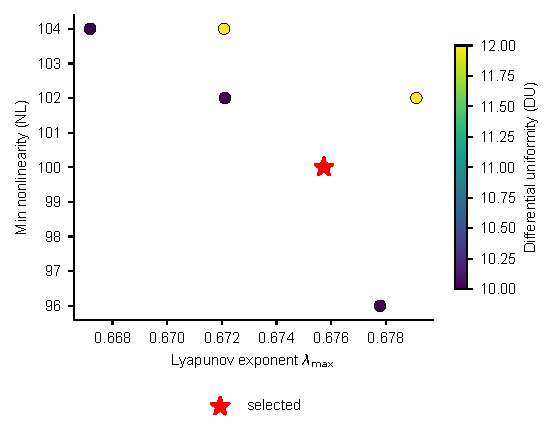
\includegraphics[width=0.85\linewidth]{figures/fig_03_pareto.pdf}
  \caption{Three-objective nondominated set for seed 42, projected
  onto largest Lyapunov exponent and minimum coordinate nonlinearity;
  color encodes differential uniformity. The red marker denotes the
  normalized-distance-to-ideal compromise selection.}
  \label{fig:pareto}
\end{figure}

\begin{figure}[ht]
  \centering
  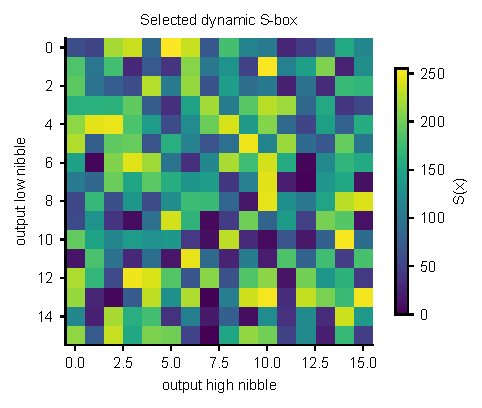
\includegraphics[width=0.85\linewidth]{figures/fig_04_sbox.pdf}
  \caption{Selected S-box reshaped as a $16 \times 16$ table.
  Every output value $0,\ldots,255$ appears exactly once
  (bijection).}
  \label{fig:sbox}
\end{figure}

\begin{figure}[ht]
  \centering
  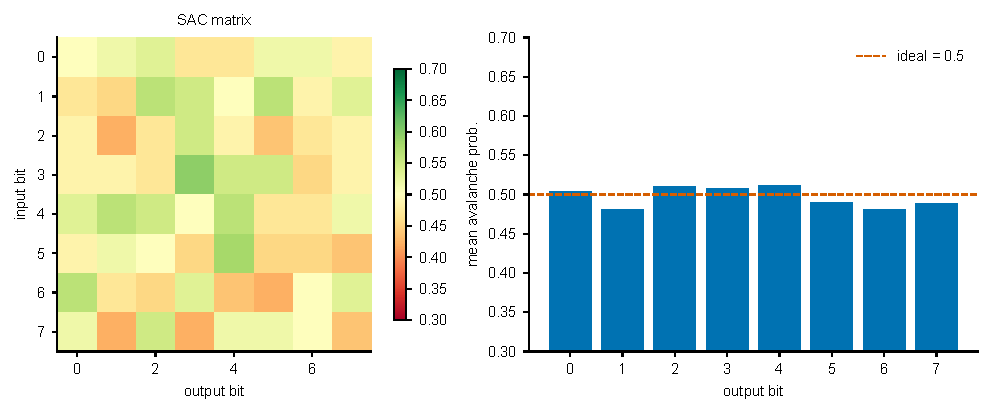
\includegraphics[width=0.85\linewidth]{figures/fig_05_sac.pdf}
  \caption{SAC matrix (left) and per-output-bit mean avalanche
  probability (right) of the seed-42 selected S-box. The dashed line
  at $0.5$ marks the ideal avalanche balance. Overall SAC is 0.4966.}
  \label{fig:sac}
\end{figure}

\begin{figure}[ht]
  \centering
  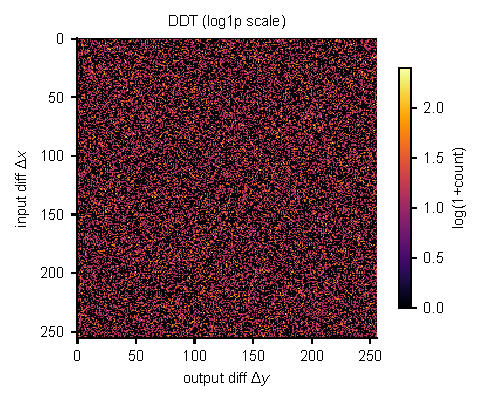
\includegraphics[width=0.85\linewidth]{figures/fig_06_ddt.pdf}
  \caption{Difference distribution table (DDT) of the selected
  S-box on a $\log(1 + \mathrm{count})$ scale. The peak DDT entry
  is $10$, defining $\mathrm{DU}=10$.}
  \label{fig:ddt}
\end{figure}

\begin{figure}[ht]
  \centering
  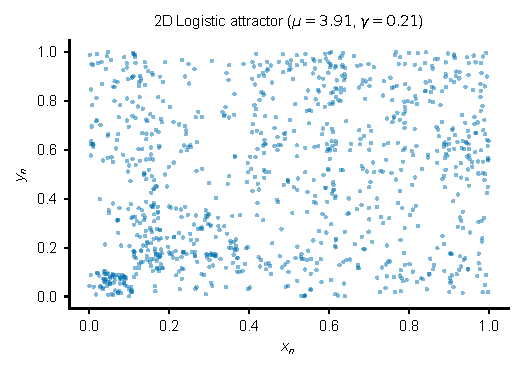
\includegraphics[width=0.85\linewidth]{figures/fig_02_attractor.pdf}
  \caption{Illustrative orbit of the modulo-one coupled Logistic map
  at $(\mu, \gamma)=(3.91,0.21)$; this is not a trajectory from a
  selected optimizer solution.}
  \label{fig:attractor}
\end{figure}

\begin{figure}[ht]
  \centering
  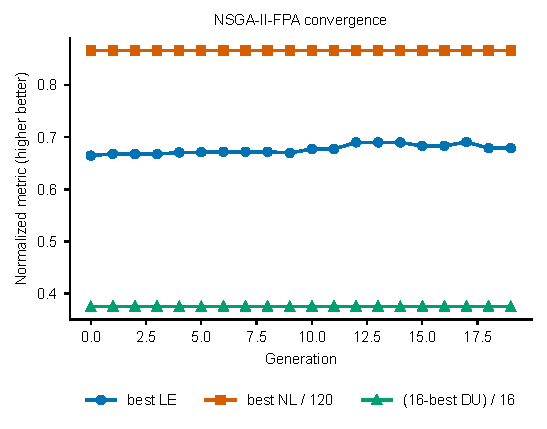
\includegraphics[width=0.85\linewidth]{figures/fig_07_convergence.pdf}
  \caption{Best-so-far largest Lyapunov exponent, minimum coordinate
  nonlinearity, and differential uniformity over 20 generations for
  the FPA run with seed 42. Values are plotted on separate normalized
  scales; the curves are descriptive and do not establish an FPA effect.}
  \label{fig:convergence}
\end{figure}

\begin{figure}[ht]
  \centering
  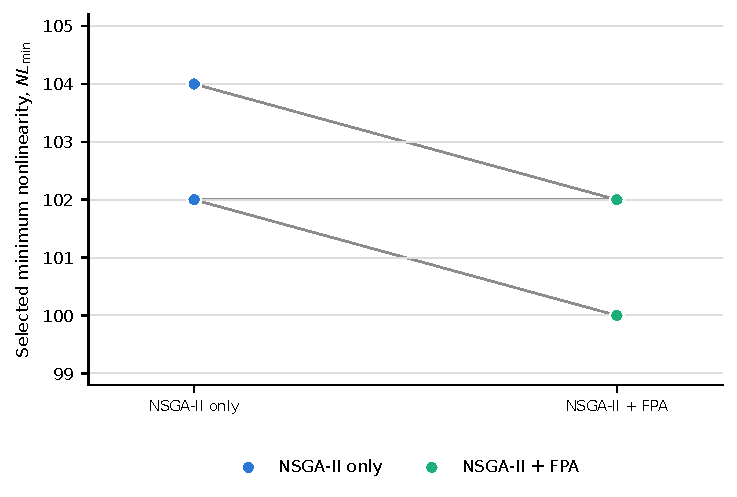
\includegraphics[width=0.72\linewidth]{figures/fig_08_paired_ablation.pdf}
  \caption{Paired selected $\mathrm{NL}_{\min}$ values for NSGA-II
  and NSGA-II with FPA perturbations across five seeds. Lines connect
  runs sharing the same initialization seed. The overlap and mixed
  directions show that this small seed set does not establish an FPA
  advantage.}
  \label{fig:ablation}
\end{figure}

\begin{table}[ht]
  \centering
  \small
  \setlength{\tabcolsep}{4pt}
  \caption{Paired five-seed optimizer comparison. Entries are mean (SD);
  $\Delta$ is FPA minus NSGA-II-only, with percentile bootstrap 95\% CI
  from 100,000 resamples of the five paired differences. Exact two-sided
  sign-flip tests were Holm-adjusted across six metrics; adjusted
  $p=0.375$ for LE and $p=1.00$ for each other metric.}
  \label{tab:ablation}
  \begin{tabular}{l c c c}
    \toprule
    Metric & FPA mean (SD) & NSGA-II mean (SD) & $\Delta$ [95\% CI] \\
    \midrule
    $\chi_{\mathrm{LE}}$ & 0.6725 (0.0029) & 0.6754 (0.0078) & $-0.00295$ [$-0.00854$, 0.00332] \\
    $\mathrm{NL}_{\min}$ & 101.6 (0.89) & 102.4 (0.89) & $-0.80$ [$-1.6$, 0.0] \\
    SAC & 0.5006 (0.0034) & 0.4982 (0.0040) & 0.00239 [$-0.00107$, 0.00605] \\
    BIC-SAC dev. & 0.0342 (0.0008) & 0.0348 (0.0016) & $-0.00067$ [$-0.00199$, 0.00066] \\
    DU & 10.0 (0.00) & 10.0 (0.00) & 0.00 [0.0, 0.0] \\
    LAP & 0.1422 (0.0065) & 0.1359 (0.0089) & 0.00625 [$-0.00469$, 0.01719] \\
    \bottomrule
  \end{tabular}
\end{table}

\end{document}














